\section{Activation} \label{sec:activation}
The activation function is a term that we repeatedly have used, but not really detailed. It is used to activate the outputs, which often need to take some certain properties. For instance, when doing classification, the outputs are probabilities and therefore between 0 and 1. A nonlinear activation function is often preferred to reinforce the non-linearity of the neural network. 

Traditionally, the logistic function and the tanh function have been used as activation functions, since they where believed to work in the same way as the human brain. However, in 2012 a new network was introduced known as AlexNet, taking image recognition to a new level. They used a function named Rectified Linear Units (ReLU), which is zero for negative values. Based on this, some successful activation functions have been innovated in the recent years, such as Leaky ReLU and Exponential Linear Unit (ELU). They will be examined one after another below. 



\iffalse
In figure (\ref{fig:activation_functions}), \textit{standard RELU, leaky RELU} and \textit{ELU} are plotted along with the logistic function.

\begin{figure} [H]
	\centering
	\subfloat[logistic]{{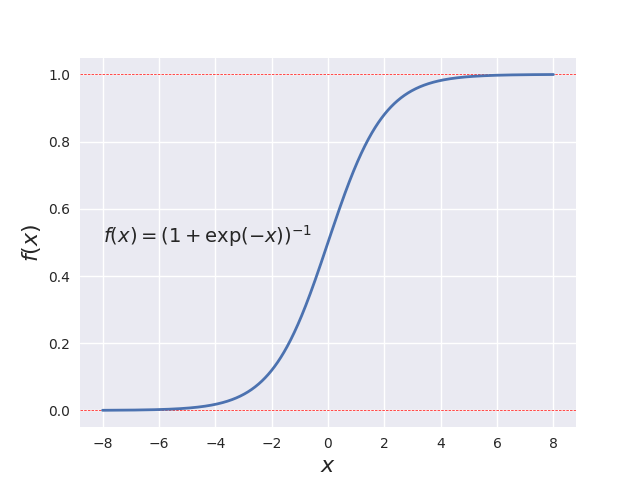
\includegraphics[width=8cm]{../plots/sigmoid.png} }}
	\subfloat[ReLU]{{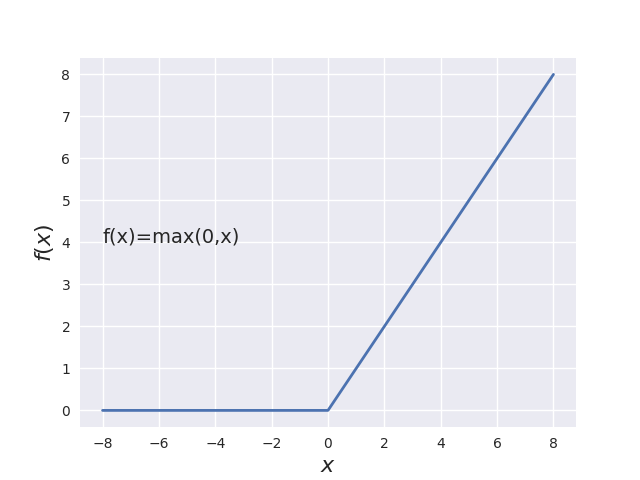
\includegraphics[width=8cm]{../plots/ReLU.png} }}\\
	
	\subfloat[Leaky ReLU]{{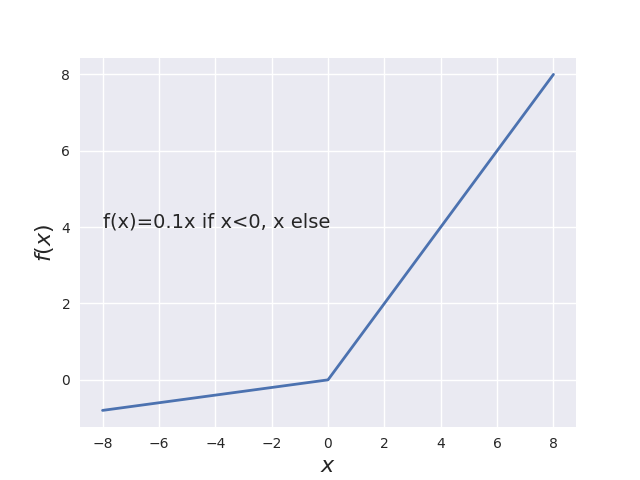
\includegraphics[width=8cm]{../plots/LeakyReLU.png} }}%
	\subfloat[ELU]{{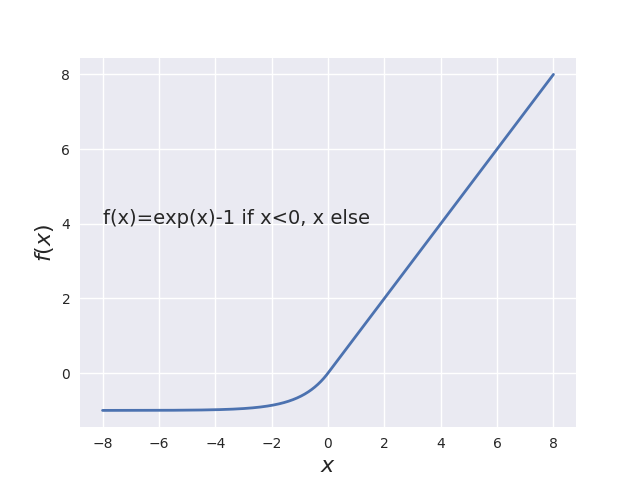
\includegraphics[width=8cm]{../plots/ELU.png} }}
	\caption{Some more or less popular activation functions}%
	\label{fig:activation_functions}%
\end{figure}
\fi

\subsection{Logistic}
The logistic activation function, also called the sigmoid function, is already mentioned several times in this report. It is widely used in classification, because it maps the outputs between 0 and 1 such that they represent probabilities for the different classes. Another important property is that 

\subsection{ReLU}

\subsection{ELU}